%!TEX program = xelatex
% 完整编译: xelatex -> biber/bibtex -> xelatex -> xelatex
\documentclass[lang=cn,a4paper,newtx,bibend=bibtex]{elegantpaper}

\title{Problems of Chapter 5}
\author{张志心 \ 混合2106}

\date{\zhdate{2023/12/20}}

% \qedhere to make the square straight after

\usepackage{array}
\usepackage{tcolorbox}
\usepackage{tikz}
\usepackage{pgfplots}
\usepackage{float}
\usepackage{bm}
\usepackage{amsmath}

\newtcolorbox{prob}[1][]{
  colframe=gray,
  colback=white,
  boxrule=1.5pt, % 控制外边框线的宽度
  sharp corners, % 使用直角边框
  fonttitle=\bfseries,
  title=#1
}

\newcommand{\ccr}[1]{\makecell{{\color{#1}\rule{1cm}{1cm}}}}
\newcommand{\xB}{\bm{x}}
\newcommand{\yB}{\bm{y}}
\newcommand{\gB}{\bm{g}}
\newcommand{\uB}{\bm{u}}
\newcommand{\vB}{\bm{v}}
\newcommand{\wB}{\bm{w}}
\newcommand{\wanwan}[1]{\tilde{#1}}
\newcommand{\dd}{\mathrm{d}}
\newcommand{\RBB}{\mathbb{R}}
\newcommand{\CBB}{\mathbb{C}}
\newcommand{\FBB}{\mathbb{F}}
\newcommand{\FM}{\mathcal{F}}
\newcommand{\SM}{\mathcal{S}}
\newcommand{\LM}{\mathcal{L}}
\newcommand{\VM}{\mathcal{V}}
\newcommand{\CM}{\mathcal{C}}
\newcommand{\upset}[2]{\stackrel{#1}{#2}}
\newcommand{\domf}{\textrm{dom}\;f}
\newcommand{\Int}[4]{\int_{#1}^{#2}{#3}{\dd {#4}}}
\newcommand{\indot}[2]{\langle {#1}, {#2} \rangle}
\newcommand{\functiontype}[3]{\FM_{#1}^{#2,#3}(\RBB^n)}
\newcommand{\normgen}[1]{\left\| #1 \right\|}
\newcommand{\strongconvextype}[2]{\SM_{#1}^{#2}(\RBB^n)}
\newcommand{\argmin}{\mathop{\rm argmin}}

\pgfplotsset{compat=1.17}

\addbibresource[location=local]{reference.bib}

\begin{document}

\maketitle

\section{Theoretical questions}

\begin{prob}[5.6.1-\textrm{I} Give a detailed proof of Theorem 5.7.]

集合 $\mathcal{C}[a, b]$ ($[a, b]$ 上全体连续函数)是 $\mathbb{C}$ 上
内积空间,内积运算定义为 $\langle  u, v \rangle = \int_a^b \rho(t)u(t)\overline{v(t)} \mathrm{d}t$。
其中 $\overline{v(t)}$ 是 $v(t)$ 的复共轭,权重函数 $\rho(x) \in \mathcal{C}[a, b]$ 满足
$\rho(x) > 0, \forall x \in [a, b]$,
且 $\| u \|_2 = \left(\int_a^b \rho(t)|u(t)|^2\mathrm{d}t\right)^{\frac12}$ 
是 $\mathcal{C}[a, b]$ 在 $\mathbb{R}$ 上的范数。

\end{prob}
\begin{proof}~~

\begin{enumerate}
\item 证明:$\mathcal{C}[a, b]$ 是 $\mathbb{C}$ 上线性空间。
\begin{enumerate}
  \item[(1)] $\mathbb{C}$ 是一个域。加法单位元为 $0$,乘法单位元为 $1$;
  \item[(2)] 交换律:$\forall \uB, \vB \in \CM[a, b], \uB + \vB = \vB + \uB$;
  \item[(3)] 加法结合律:$\forall \uB, \vB, \wB \in \CM[a, b], (\uB + \vB) + \wB = \uB + (\vB + \wB)$;
  \item[(4)] 乘法结合律:$\forall \uB \in \CM[a, b], \forall a, b \in \CBB, (ab)\uB = a(b\uB)$;
  \item[(5)] 加法单位元:$\bm{0}(x) \equiv \bm{0} \in \CM[a, b], \forall \uB \in \CM[a, b], \uB + 0 = 0 + \uB = \uB$;
  \item[(6)] 加法逆元:$\forall \uB \in \CM[a, b]$,令 $\vB(t) = -\uB(t) \in \CM[a, b]$, 满足 $\vB + \uB = \uB + \vB = 0$;
  \item[(7)] 乘法单位元:$\forall u \in \CM[a, b], 1\uB(t) = 1\times\uB(t) = \uB \Rightarrow 1\uB = \uB$;
  \item[(7)] 分配律:$\forall \uB, \vB \in \CM[a, b], \forall a, b\in \CBB, \begin{cases} (a+b)\uB = a\uB + b\uB, \\ a(\uB + \vB) = a\uB + b\vB.\end{cases}$  
\end{enumerate}
\item 证明:$\langle \cdot, \cdot \rangle$ 是内积运算,$\mathcal{C}[a, b]$ 是 $\mathbb{C}$ 上内积空间。

$\forall \uB, \vB, \wB \in \CM[a, b], \lambda \in \CBB$:
\begin{enumerate}
  \item[(1)] 正定性:$\langle \uB, \uB \rangle = \int_a^b \rho(t)\uB(t)\overline{\uB(t)}\dd t = \int_a^b \rho(t)|\uB(t)|^2 \dd t \ge 0$;
  \item[(2)] 绝对性:若 $\langle \uB, \uB \rangle = \int_a^b \rho(t)|\uB(t)|^2 \dd t = 0$,因为 $\rho(t) > 0, \uB(t) \in \CM[a, b]$,所以 $\uB(t) \equiv 0$;
  \item[(3)] 线性性:$\lambda \langle \uB + \vB, \wB \rangle = \int_a^b \rho(t)(\lambda \uB(t) + \vB(t))\overline{\wB(t)} \dd t = \lambda \int_a^b \rho(t)\uB(t)\overline{\wB(t)}\dd t + \int_a^b \rho(t)\vB(t)\overline{\wB(t)} \dd t = \lambda \langle \uB, \wB\rangle + \langle \vB, \wB \rangle$;
  \item[(4)] 共轭对称性:$\langle \vB, \uB \rangle = \int_a^b \rho(t)\vB(t)\overline{\uB(t)}\dd t = \int_a^b \overline{\rho(t)\uB(t)\overline{\vB(t)}}\dd t = \overline{\langle \uB, \vB\rangle}$. 
\end{enumerate}
\item 证明:$\| u \|_2$ 是 $\mathcal{C}[a, b]$ 在 $\mathbb{R}$ 上范数。

根据定义,$\| \cdot \|_2 $ 为一个映射 $\CM[a, b] \to \RBB$: $\| \uB \|_2 = \sqrt{\langle \uB, \uB \rangle} =  \left(\int_a^b \rho(t)|u(t)|^2\mathrm{d}t\right)^{\frac12}, \forall \uB \in \CM[a, b]$。
\end{enumerate}

\end{proof}

\begin{prob}[5.6.1-\textrm{II}]
Consider the Chebyshev polynomials of the first kind.

\begin{enumerate}
  \item[(a)] Show that they are orthogonal on $[-1, 1]$ with respect to the 
              inner product in Theorem 5.7 with the weight function $\rho(x) = \frac{1}{\sqrt{1 - x^2}}$.
  \item[(b)] Normalize the first three Chebyshev polynomials to arrive at an orthogonal system.
\end{enumerate}
\end{prob}

\begin{solution} ~~

\begin{enumerate}
\item[(a)]
\begin{equation*}
\begin{aligned}
  \langle T_n, T_m \rangle &= \int_{-1}^1 \rho(t) T_n(t) T_m(t) \dd t 
  = \int_{-1}^1 \frac{1}{\sqrt{1 - x^2}} \cos (n \arccos t)\cos (m \arccos t) \dd t \\
  &= - \int_{-1}^1 \cos (n \arccos t) \cos (m \arccos t) \dd \arccos t \\
  &= \int_0^{\pi} \cos (n \theta) \cos (m \theta) \dd \theta 
  = \int_0^{\pi} \dfrac{\cos [(n - m) \theta] + \cos [(n + m)\theta]}{2} \dd \theta \\
  &= \begin{cases}
      \left(\dfrac{\sin [(n - m) \theta]}{2(n - m)} + \dfrac{\sin [(n + m) \theta]}{2(n + m)} \right)\bigg |_0^{\pi} &(n \neq m)\\
      \left(\dfrac{\theta}2 + \dfrac{\sin 2n\theta}{4n}\right) \bigg|_0^{\pi} & (n = m \neq 0)\\
      \theta \big|_0^{\pi} & (n = m = 0)
  \end{cases} 
  = \begin{cases}
    0 & (n \neq m) \\
    \frac{\pi}2 & (n = m \neq 0)\\
    \pi & (n = m = 0)
\end{cases} 
\end{aligned}
\end{equation*}
所以 $\{T_n\}$ 正交。
\item[(b)]
$\| T_n \|_2^2 = \langle T_n, T_n \rangle = \begin{cases} \frac{\pi}2 & n \neq 0 \\ \pi & n = 0\end{cases}$,

$T_0(x) = 1, T_1(x) = x, T_2(x) = 2x^2 - 1$,

所以对于 $\{T_0, T_1, T_2\}$,标准正交基为 $\left\{\sqrt{\frac1{\pi}}, \sqrt{\frac2{\pi}} x, \sqrt{\frac2{\pi}} (2x^2 - 1)\right\}$。

\end{enumerate}
\end{solution}

\begin{prob}[5.6.1-\textrm{III} 连续函数的最小平方估计]
  Least-square approximation of a continuous function.
  Approximate the circular arc given by the equation
  $y(x) = \sqrt{1 - x^2}$ for $x \in [−1, 1]$ by a quadratic polynomial
  with respect to the inner product in Theorem 5.7.
  \begin{enumerate}
    \item[(a)] $\rho(x) = \frac{1}{\sqrt{1 - x^2}}$ with Fourier expansion,
    \item[(b)] $\rho(x) = \frac{1}{\sqrt{1 - x^2}}$ with normal equations.
  \end{enumerate}
\end{prob}

\begin{solution} ~~

\begin{enumerate}
\item[(a)] 
\begin{equation*}
\begin{aligned}
  &\indot{y}{T_0^*} = \indot{y}{\sqrt{\frac1{\pi}}} = \sqrt{\frac{1}{\pi}} \int_{-1}^1 \frac{1}{\sqrt{1 - t^2}} \sqrt{1 - t^2} \dd t = 2 \sqrt{\frac{1}{\pi}} \\
  &\indot{y}{T_1^*} = \indot{y}{\sqrt{\frac2{\pi}}x} = \sqrt{\frac{2}{\pi}} \int_{-1}^1 \frac{1}{\sqrt{1 - t^2}} \sqrt{1 - t^2} t \dd t = 0 \\
  &\indot{y}{T_2^*} = \indot{y}{\sqrt{\frac2{\pi}}(2x^2 - 1)} = \sqrt{\frac{2}{\pi}} \int_{-1}^1 \frac{1}{\sqrt{1 - t^2}}\sqrt{1 - t^2} 2t^2 - 1 \dd t = - \frac23 \sqrt{\frac2{\pi}}
\end{aligned}
\end{equation*}
所以 $\hat{y}(x) = 2\sqrt{\frac1{\pi}}\cdot\sqrt{\frac{1}{\pi}} - \frac23 \sqrt{\frac{2}{\pi}}\cdot\sqrt{\frac{2}{\pi}}(2x^2 - 1) = \dfrac{10 - 8x^2}{3\pi}$。
\item[(b)]
$\indot{1}{1} = \int_{-1}^{1} \frac{1}{\sqrt{1 - x^2}} \dd x = \arccos x \big|_{-1}^1 = \pi$,

$\indot{1}{x} = \Int{-1}{1}{\frac{x}{\sqrt{1 - x^2}}}{x} = 0$。

$\indot{x}{x} = \indot{1}{x^2} = \Int{-1}{1}{\frac{x^2}{\sqrt{1-x^2}}}{x}\upset{x = \cos \theta}{=} - \Int{0}{\pi}{\frac{\cos^2 \theta}{\sin \theta}}{\cos \theta} = \Int{0}{\pi}{\cos^2 \theta}{\theta} = \frac{\pi}2$,

$\indot{x}{x^2} = \Int{-1}{1}{\frac{x^3}{\sqrt{1 - x^2}}}{x} = 0$,

$\indot{x^2}{x^2} = \Int{-1}{1}{\frac{x^4}{\sqrt{1 - x^2}}}{x}\upset{x =\cos \theta}{=} -\Int{0}{\pi}{\frac{\cos^4\theta}{\sin \theta}}{\cos \theta}=\Int{0}{\pi}{\cos^4 \theta}{\theta} = \frac{3\pi}8$。
\[
  G(1, x, x^2) = \begin{bmatrix}
    \indot{1}{1} & \indot{1}{x} & \indot{1}{x^2} \\
    \indot{x}{1} & \indot{x}{x} & \indot{x}{x^2} \\
    \indot{x^2}{1} & \indot{x^2}{x} & \indot{x^2}{x^2}
  \end{bmatrix}
   = \begin{bmatrix}
    \pi & 0 & \frac{\pi}2 \\
    0 & \frac{\pi}2 & 0  \\
    \frac{\pi}2 & 0 & \frac{3\pi}8
  \end{bmatrix}
\]

$\left[\indot{y}{1}, \indot{y}{x}, \indot{y}{x^2} \right]^{\mathrm{T}} = \left[\Int{-1}{1}{}{x}, \Int{-1}{1}{x}{x}, \Int{-1}{1}{x^2}{x}\right]^{\mathrm{T}} = \left[2, 0, \frac{2}{3}\right]^{\mathrm{T}}$。

\[
  \begin{bmatrix}
    \pi & 0 & \frac{\pi}2 \\
    0 & \frac{\pi}2 & 0  \\
    \frac{\pi}2 & 0 & \frac{3\pi}8
  \end{bmatrix}
  \begin{bmatrix}
    a_0 \\ a_1 \\ a_2
  \end{bmatrix}
  = \begin{bmatrix}
    2 \\ 0 \\ \frac23
  \end{bmatrix}
  \Rightarrow
  \begin{bmatrix}
    a_0 \\ a_1 \\ a_2
  \end{bmatrix}
  = \begin{bmatrix}
    \frac{10}{3\pi} \\ 0 \\ -\frac{8}{3\pi}
  \end{bmatrix}
\]

所以 $\hat{y}(x) = \dfrac{10 - 8x^2}{3\pi}$。

\end{enumerate}
\end{solution}

\begin{prob}[5.6.1-\textrm{IV} 用正交多项式进行离散最小二乘估计]
  Discrete least square via orthonormal polynomials.
  Consider the example on the table of sales record in Example 5.49.
\begin{enumerate}
  \item[(a)] Starting from the independent list $(1, x, x^2)$, construct orthonormal
  polynomials by the Gram-Schmidt process using
  \[\langle u(t), v(t) \rangle = \sum_{i = 1}^{N} \rho(t_i)u(t_i)v(t_i).\]
  as the inner product with $N = 12$ and $\rho(x) = 1$.
  \item[(b)] Find the best approximation $\hat{\varphi} = \sum_{i = 0}^2 a_i x^i$ such that
  $\| y - \hat{\varphi}\| \le \| y - \sum_{i = 0}^2 b_i x^i\|$ for all $b_i \in \mathbb{R}$.
  Verify that $\hat{\varphi}$ is that same as that of the example on the table of sales record
  in the notes.
  \item[(c)] Suppose there are other tables of sales record in
  the same format as that in the example. Values
  of $N$ and $x_i$’s are the same, but the values of $y_i$’s
  are different. Which of the above calculations can
  be reused? Which cannot be reused? What advantage of orthonormal polynomials
  over normal equations does this reuse imple?
\end{enumerate}
\end{prob}

\begin{solution}~~

\begin{enumerate}
\item[(a)]
$\{u_0, u_1, u_2\} = \{1, x, x^2\}$。

$\indot{u_0}{u_0} = \indot{1}{1} = \sum\limits_{i = 1}^{12} 1 = 12 \Rightarrow u_0^* = \frac{u_0}{\| u_0 \|_2} = \frac1{2\sqrt{3}}$;

$\indot{u_0^*}{u_1} = \frac{1}{2\sqrt{3}} \sum\limits_{i = 1}^{12} x_i = \frac{78}{2\sqrt{3}}$,

$v_1 = u_1 - \indot{u_0^*}{u_1} u_0^* = x - \frac{13}2$,$\indot{v_1}{v_1} = \sum\limits_{i = 1}^{12} (x_i - \frac{13}2)^2 = 143 \Rightarrow u_1^* = \frac{v_1}{\| u_1\|_2} = \frac{x - \frac{13}2}{\sqrt{143}}$;

$\indot{u_0^*}{u_2} = \frac1{2\sqrt{3}}\sum\limits_{i = 1}^{12} x_i^2 = \frac{650}{2\sqrt{3}}$,
$\indot{u_1^*}{u_2} = \frac{1}{\sqrt{143}}\sum\limits_{i = 1}^{12} (x_i - \frac{13}2)x_i^2 = \frac{1859}{\sqrt{143}}$,

$v_2 = u_2 - \indot{u_0^*}{u_2}u_0^* - \indot{u_1^*}{u_2}u_1^* = x^2 - 13x + \frac{91}3$,
$\indot{v_2}{v_2} = \sum\limits_{i = 1}^{12}(x_i^2 - 13x_i + \frac{91}3)^2 = \frac{4004}{3}$

$\Rightarrow u_2^* = \frac{v_2}{\| u_2\|_2} =\sqrt{\frac{3}{4004}}(x^2 - 13x + \frac{91}{3})$。


所以,一组标准正交基为 $\left\{\frac{1}{2\sqrt3}, \frac{2x - 13}{2 \sqrt{143}}, \sqrt{\frac3{4004}}(x^2 - 13x + \frac{91}3)\right\}$。


\item[(b)]
$\indot{u_0^*}{y}=\sum\limits_{i=1}^{12}\frac{y_i}{2\sqrt 3}=277\sqrt 3$,
$\indot{u_1^*}{y}=\sum\limits_{i=1}^{12}\frac{y_i(2x_i-13)}{2\sqrt {143}}=\dfrac{589}{\sqrt {143}}$,

$\indot{u_2^*}{y}=\sum\limits_{i=1}^{12}{\sqrt{\frac{3}{4004}}}{y_i(x_i^2-13x_i+\frac{91}{3})}={12068}{\sqrt{\frac{3}{4004}}}$,

所以 $\hat{\varphi} = \indot{u_0^*}{y}u_0^* + \indot{u_1^*}{y}u_1^* + \indot{u_2^*}{y}u_2^* = 9.04196 x^2 - 113.427 x + 386.000$,,与给出的结果一致。

\item[(c)] 
标准正交基$\{u_0^*, u_1^*, u_2^*\}$不需要重新计算,需要重新计算 $\indot{u_0^*}{y}, \indot{u_1^*}{y}, \indot{u_2^*}{y}$ 需要重新计算。

若需要基于 $n$ 个给定点值拟合 $p$ 次多项式,有 $q$ 个需要拟合的多项式(使用 $\{x_i\}$ 相同的数据),

若使用标准正交基的方法,
首先使用 $O(np^2)$ 次运算得出标准正交基 $\{u_i^*\}_{i = 0}^{p}$,然后对于每组数据,需要 $O(np)$ 次运算得到 $\{\indot{u_i^*}{y}\}_{i = 0}^{p}$。
总共需要的时间复杂度为 $O(np^2 + qnp)$。

若使用正则方程组的方法,
首先需要 $O(np^2)$ 次运算得到 $G(1, x, \cdots, x^p)$,然后对于不同的 $y$,需要用 $O(np)$ 次运算得到 $\{\indot{x^i}{y}\}_{i = 0}^p$,最后还需要 $O(p^3)$ 次运算求解方程组。
总共需要的时间复杂度为 $O(np^2 + q(np + p^3))$。

可以发现,当 $p$ 较大的时候,后者运算复杂度远高于前者。 

\end{enumerate}
\end{solution}

\begin{prob}[5.6.1-\textrm{V} Prove Theorem 5.60 and Lemma 5.61.]
  The pseudo-inverse in Definition 5.59 has the following properties.

    (PDI-1) $AA^+$ maps all columns of A to themselves: $AA^+A = A$;
    
    (PDI-2) $A^+$ acts like a weak inverse: $A^+AA^+ = A^+$;
    
    (PDI-3) Both $AA^+$ and $A^+A$ are Hermitian: $(AA^+)^* = AA^+, (A^+A)^* = A^+A.$


  If A has linearly independent columns, then $A^*A$ is invertible and we have
  \[A^+ = (A^*A)^{-1}A^*,\]
  which is then a \textit{left inverse}, i.e. $A^+A = I$. Similarly, if $A$
  has linearly independent rows, then \[A^+ = A^*(AA^*)^{-1},\] which is then a 
  \textit{right inverse}, i.e. $AA^+ = I$.
\end{prob}

\begin{proof}
  设 $A$ 的奇异值分解是 $A = U\Sigma V^*, U = (u_1, \cdots, u_m), V = (v_1, \cdots, v_n)$,
  $\Sigma = \begin{bmatrix}
    \begin{array}{ccc|c}
      \sigma_1 & & & \\
      & \ddots & & 0 \\
      & & \sigma_r & \\
      \hline
      & 0 & & 0 \\
    \end{array}
  \end{bmatrix}_{m\times n}
  $。
  则 $A^+ = V\Sigma^+U^*$, 
  $\Sigma^+ = \begin{bmatrix}
    \begin{array}{ccc|c}
      \sigma_1^{-1} & & & \\
      & \ddots & & 0 \\
      & & \sigma_r^{-1} & \\
      \hline
      & 0 & & 0 \\
    \end{array}
  \end{bmatrix}_{n\times m}
  $。$\Sigma\Sigma^+ = \begin{bmatrix}
    I & 0 \\ 0 & 0 
  \end{bmatrix}_{m\times m}$,
  $\Sigma\Sigma^+\Sigma = \Sigma$,
  $\Sigma^+\Sigma = \begin{bmatrix}
    I & 0 \\ 0 & 0 
  \end{bmatrix}_{n\times n}$,
  $\Sigma^+\Sigma\Sigma^+ = \Sigma^+$。

  (PDI-1) $AA^+A = (U\Sigma V^*)(V\Sigma^+ U^*)(U\Sigma V^*) = U\Sigma\Sigma^+\Sigma V^* = U\Sigma V^* = A$;
  
  (PDI-2) $A^+AA^+ = (V\Sigma^+U^*)(U\Sigma V^*)(V\Sigma^+U^*) = V\Sigma^+\Sigma\Sigma^+ U^* = V\Sigma^+U^* = A^+$;

  (PDI-3) $(AA^+)^* = ((U\Sigma V^*)(V\Sigma^+U^*))^* = (U\Sigma\Sigma^+U^*)^* = U(\Sigma\Sigma^+)U^* = U\Sigma\Sigma^+U^* = AA^+,$
          
  ~~~~~~~~~~~~~~$(A^+A)^* = ((V\Sigma^+U^*)(U\Sigma V^*))^* = V(\Sigma^+\Sigma^*)V^* = V\Sigma^+\Sigma V^* = A^+A$。

  $(A^*A)^{-1}A^* = ((U\Sigma V^*)^*(U\Sigma V^*))^{-1}(U\Sigma V^*)^* = (V\Sigma^*\Sigma V^*)^{-1}V\Sigma^* U$,因为 $A$ 列满秩,所以 $r = n$,
  
  $\Sigma = \begin{bmatrix}
    \begin{array}{ccc}
      \sigma_1 & & \\
      & \ddots & \\
      & & \sigma_n \\
      \hline
      & 0 &
    \end{array}
  \end{bmatrix}_{m\times n}
  $, $\Sigma^*\Sigma = \begin{bmatrix}
    \sigma_1^2 & & \\
    & \ddots & \\
     & & \sigma_n^2
  \end{bmatrix}$, 
  $(\Sigma^*\Sigma)^{-1}\Sigma^* = \Sigma^+$.

  所以 
  $(A^*A)^{-1}A^* = V(\Sigma^*\Sigma)^{-1}V^*V\Sigma^*U^* = V(\Sigma^*\Sigma)^{-1}\Sigma^*U^* = V\Sigma^+U^* = A^+ \Rightarrow A^+A = I$。


  $A^*(AA^*)^{-1} = A^*((U\Sigma V^*)(U\Sigma V^*)^*)^{-1} = A^*(U\Sigma \Sigma^* U^*)^{-1}$,因为 $A$ 行满秩,所以 $r = m$,

  $\Sigma = \begin{bmatrix} 
    \begin{array}{ccc|c}
      \sigma_1 & & & \\
       & \ddots & & 0\\
       & & \sigma_n & 
    \end{array}
  \end{bmatrix}_{m\times n}$,
  $\Sigma\Sigma^* = \begin{bmatrix}
    \sigma_1^2 & & \\
    & \ddots & \\
     & & \sigma_m^2
  \end{bmatrix}$, $\Sigma^*(\Sigma\Sigma^*)^{-1} = \Sigma^+$,

  所以 $A^*(AA^*)^{-1} = (U\Sigma V^*)^*U(\Sigma \Sigma^*)^{-1}U^* = V\Sigma^*(\Sigma\Sigma^*)^{-1}U^* = V\Sigma^+U^* = A^+ \Rightarrow AA^+ = I$。
\end{proof}

\section{Programming assignments}

使用 \lstinline{make all + make run} 运行得到所有结果。

\subsection{A.}

使用正则方程组计算结果为:$2.17572 + 2.67041 x -0.238444 x^2$。
其中
\[
  G = \begin{bmatrix}
    21 & 105 & 717.5 \\
    105 & 717.5 & 5512.5 \\
    717.5 & 5512.5 & 45166.6 \\
\end{bmatrix}
\]

二条件数 $\kappa(G) = \|G\|_2\|G^{-1}\|_2 = 18981.08307675254$。

\begin{figure}[H]
  \centering
  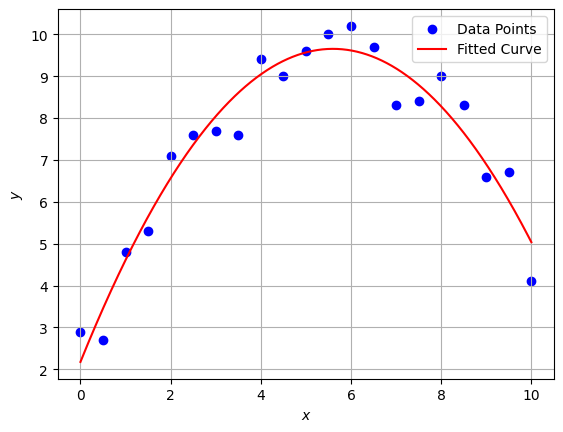
\includegraphics[width=0.8\linewidth]{output.png}
\end{figure}

\subsection{B.}

使用正交分解法计算结果为:$2.17572 + 2.67041 x -0.238444 x^2$。
其中
\[
  R_1 = \begin{bmatrix}
    -4.58258 & -22.9129 & -156.571 \\
    0 & 13.8744 & 138.744 \\
    0 & 0 & -37.4438 \\
\end{bmatrix}
\]

二条件数 $\kappa(R_1) = 137.77147945973786$

矩阵的条件数反映了方程组的稳定性,进而反映了算法的稳定性。因
此,正交分解的稳定性比正则化方程组要好。

\subsection{C.}

\begin{enumerate}
\item 证明 
$\forall j = 0, 1, \cdots, n, \sum_{k = 0}^{n} \dfrac{\alpha_k}{j + k + 1} = \int_0^1 f(x)x^j \dd x, f(x) = \frac{1}{1 + x}$,
的解为如下形式:
\[\forall j = 0, 1, \cdots, n, \alpha_j = \beta_j \ln 2 + \gamma_j, \beta_j, \gamma_j \in \mathbb{Q}.\]

\begin{proof}
  根据题意,$G = \{\indot{x^j}{x^k}\}_{(n + 1)\times (n + 1)} = \{\frac{1}{j+k+1}\}_{(n+1)\times(n+1)}\in \mathbb{Q}^{(n+1)\times(n+1)}, j,k = 0, \cdots n$,
  方程组的右端项 $r_j := \Int{0}{1}{\dfrac{x^j}{1+x}}{x} = (-1)^j\ln 2 + \sum\limits_{i=1}^{j} (-1)^{i+j} \frac1i \in \mathbb{Q} + \mathbb{Q}\ln2$。
  因为 $G\in \mathbb{Q}^{(n+1)*(n+1)}$,
  Hilbert 矩阵可逆,所以 $G^{-1} \in \mathbb{Q}^{(n+1)\times(n+1)}$。
  所以 $[\alpha_0, \cdots, \alpha_n]^T = G^{-1} [r_0, \cdots, r_n]^T \in \mathbb{Q} + \mathbb{Q}\ln2$。
\end{proof}

\item 使用高斯消元分别求解 $\beta_j, \gamma_j, j = 0, \cdots, n$,$n$ 取遍 $1, 2, \cdots, 6$。
      输出结果见 \lstinline{data/resC.txt}。

\item 计算 $\alpha_j = \beta_j \ln 2 + \gamma_j$ 得到结果如下:

\begin{table}[h]
  \centering
  \begin{tabular}{|c|c|c|c|c|c|c|}
  \hline
  $\beta \ln(2) + \gamma$ & $n = 1$ & $n = 2$ & $n = 3$ & $n = 4$ & $n = 5$ & $n = 6$ \\
  \hline
  $\alpha_0$ & 0.931472 & 0.986039 & 0.997279 & 0.999483 & 0.999904 & 0.999982 \\
  $\alpha_1$ & -0.476649 & -0.80405 & -0.938929 & -0.983022 & -0.995633 & -0.998938 \\
  $\alpha_2$ && 0.3274 & 0.664599 & 0.863017 & 0.951295 & 0.984346 \\
  $\alpha_3$ &&& -0.224799 & -0.533448 & -0.768857 & -0.901063 \\
  $\alpha_4$ &&&& 0.154325 & 0.41916 & 0.667044 \\
  $\alpha_5$ &&&&& -0.105934 & -0.324072 \\
  $\alpha_6$ &&&&&& 0.0727128 \\
  \hline
  \end{tabular}
  \end{table}

  横向观察,可以看出 $a_0, a_1, a_2, a_3$ 都分别收敛到了 $(-1)^j$,
  说明该计算有较好的收敛性质。

\item 直接带入 $\ln 2$ 的估计值计算 $\alpha_j$ 的值的结果如下:

\begin{table}[h]
  \centering
  \begin{tabular}{|c|c|c|c|c|c|c|}
  \hline
   & $n = 1$ & $n = 2$ & $n = 3$ & $n = 4$ & $n = 5$ & $n = 6$ \\
  \hline
  $\alpha_0$ & 0.9315 & 0.98625 & 0.998733 & 1.00908 & 1.0617 & 1.39125 \\
  $\alpha_1$ & -0.4767 & -0.8052 & -0.955 & -1.162 & -2.7405 & -16.5816 \\
  $\alpha_2$ & & 0.3285 & 0.703 & 1.6345 & 12.684 & 151.095 \\
  $\alpha_3$ & & & -0.249667 & -1.69867 & -31.164 & -584.808 \\
  $\alpha_4$ & & & & 0.7245 & 33.873 & 1071.96 \\
  $\alpha_5$ & & & & & -13.2594 & -926.772 \\
  $\alpha_6$ & & & & & & 304.504 \\
  \hline
  \end{tabular}
  \end{table}

可以看出并没有收敛,这是因为 Hilbert 矩阵的条件数过大(当 $n\ge 3$ 之后),方程组不稳定,因此计算误差很大。
另外使用 $\ln(2)$ 的近似值代替 $\ln(2)$ 也带来了较大的误差。

\begin{table}[H]
  \centering
  \begin{tabular}{|c|c|}
  \hline
  Hilbert Matrices & Condition Number \\
  \hline
  $H_1$ & 19.281544936250604 \\
  $H_2$ & 524.1012332900597 \\
  $H_3$ & 15571.82395090834 \\
  $H_4$ & 551998.6957924255 \\
  $H_5$ & 7711391.7485829005 \\
  $H_6$ & 6894039.332923305 \\
  \hline
  \end{tabular}
  \end{table}
  \item 使用 Tikhonov Regulation 得到的结果如下:
  \begin{table}[h]
    \centering
    \begin{tabular}{|c|c|c|c|c|c|c|}
    \hline
    & $n = 1$ & $n = 2$ & $n = 3$ & $n = 4$ & $n = 5$ & $n = 6$ \\
    \hline
    $\alpha_0$ & 0.9315 & 0.986248 & 0.998416 & 0.994862 & 0.995676 & 0.997988 \\
    $\alpha_1$ & -0.4767 & -0.805191 & -0.951424 & -0.893607 & -0.908099 & -0.938697 \\
    $\alpha_2$ & & 0.328491 & 0.694393 & 0.471413 & 0.523036 & 0.582433 \\
    $\alpha_3$ & & & -0.244072 & 0.0631045 & 0.0247755 & 0.0801941 \\
    $\alpha_4$ & & & & -0.139109 & -0.182563 & -0.250542 \\
    $\alpha_5$ & & & & & 0.0449797 & -0.165638 \\
    $\alpha_6$ & & & & & & 0.196227 \\
    \hline
    \end{tabular}
    \end{table}

    横向观察,可以看出至少 $a_0, a_1$ 都恢复了收敛性。
    
\end{enumerate}

\end{document}